\documentclass[twocolumn,10pt]{article}

\usepackage[margin=2cm]{geometry}
\usepackage{amsmath,amssymb,bm}
\usepackage{graphicx}
\usepackage{booktabs}
\usepackage{xcolor}
\usepackage{microtype}
\usepackage{authblk}
\usepackage[hidelinks]{hyperref}
% --------------------------------------------------------------------------
% BEFORE SUBMISSION: every \needspaste{} below must be resolved.
%   grep -n needspaste *.tex
% They render in red in the PDF so they cannot be missed on a read-through.
\newcommand{\needspaste}[1]{{\color{red}\textbf{[NEED TO PASTE: #1]}}}

\graphicspath{{figures/}}

% --------------------------------------------------------------------------
\title{\textbf{Physics-Informed Early Warning of Entanglement Decoherence
in Two-Qubit Systems}}

\author[1]{}
\affil[1]{\needspaste{confirm this affiliation or replace it}}
\date{}
% --------------------------------------------------------------------------

\begin{document}
\maketitle

% --------------------------------------------------------------------------
\begin{abstract}
We extend the physics-informed residual BiLSTM of
\cite{Paper1Brusnikin} to two-qubit systems with XXZ and TFIM
Hamiltonians under unknown time-dependent amplitude damping, and ask
whether its conclusions transfer.
All results are replicated across three seeds.
The slope-based physics estimate is structurally wrong when two-qubit
coherence oscillates. A pure Transformer is the best model on both
systems ($R^2 = 0.843 \pm 0.028$ on XXZ, $0.699 \pm 0.045$ on TFIM,
single-scenario training) and beats both BiLSTM variants in every seed,
by $0.01$--$0.06$; the residual model does not improve on the same BiLSTM
without the prior, and on TFIM it is worse in every seed.
A single Transformer trained on both systems with a 20-step window
reaches $R^2 = 0.814 \pm 0.034$ and $0.703 \pm 0.034$, with alarm AUROC
$0.931$ and $0.904$; a shorter window beats a longer one on both metrics
in every seed.
Measurement noise of $\sigma = 0.10$ lowers the alarm AUROC in every seed
($-0.078 \pm 0.037$), while its effect on $R^2$ is not resolved
($-0.074 \pm 0.126$).
On TFIM, predictability falls as the coupling $J$ grows and then
saturates, with no feature at the nominal transition $J = h$.
We trace this decline to the target rather than the dynamics: $T_2$ is
the first $1/e$ crossing of $\ell_1$-coherence in the computational
basis, which the TFIM Hamiltonian rotates by an angle
$\tan 2\theta = J/2h$; the resulting unitary modulation makes the
crossing time depend on the oscillation phase. The fraction of
trajectories whose coherence re-crosses the threshold tracks the loss in
$R^2$ across $J$ ($r = -0.78$), while the XXZ model, whose mixing angle
does not depend on $J$, shows neither effect.
Retraining the coupling sweep with $T_2$ defined in the energy
eigenbasis confirms it: over eight seeds the drop in $R^2$ from weak to
strong coupling falls from $0.158 \pm 0.066$ (positive in every seed) to
$0.020 \pm 0.072$, and the error no longer grows with $J$.
\end{abstract}

% --------------------------------------------------------------------------
\section{Introduction}

In \cite{Paper1Brusnikin} we showed that, for a single qubit under
unknown time-dependent dissipation, a residual model that adds a learned
correction $\delta T$ to the slope-based estimate of the decoherence
time recovers the analytic limit at constant dissipation and, when the
rate varies, improves both on the bare formula and on the same network
without the estimate.
Here we ask whether this carries over to two qubits.
Three things change.

\begin{enumerate}
  \item \textbf{Non-exponential coherence.}
    With an interaction Hamiltonian that is not diagonal in the
    computational basis, unitary evolution moves amplitude between basis
    states, so the $\ell_1$-coherence oscillates on top of its
    dissipative decay and can increase within an observation window.
    The slope-based estimate assumes it does not.
  \item \textbf{Partial observation.}
    The model sees the six single-qubit Pauli expectations, coherence
    and purity, but no two-body correlators; the two local Bloch vectors
    do not determine the two-qubit state.
  \item \textbf{Entanglement.}
    Two-qubit entanglement can vanish in finite time under purely local
    damping \cite{YuEberly2009}, so the joint decay need not follow the
    asymptotic exponential of either qubit alone.
\end{enumerate}

\subsection*{Scenarios}

Both scenarios (Table~\ref{tab:scenarios2}) use per-qubit $\sigma_-$
jump operators with the Bernstein $\gamma(t)$ parameterisation of
\cite{Paper1Brusnikin}: degree-4 polynomials with non-negative
coefficients bounded by $\gamma \leq 0.8$, cycling through six profile
shapes (random, monotone increasing, monotone decreasing, peak, step-up,
step-down).
The dynamics is the two-qubit Lindblad equation ($\hbar = 1$)
\begin{equation}
  \dot\rho = -i[H,\rho]
  + \sum_{k=1}^{2} \gamma(t)\!\left(
      L_k \rho L_k^\dagger
      - \tfrac{1}{2}\{L_k^\dagger L_k, \rho\}\right),
  \label{eq:lindblad2}
\end{equation}
with $L_1 = \sigma_-\otimes I$ and $L_2 = I\otimes\sigma_-$, integrated
with \textsc{QuTiP}~\cite{qutip} \cite{Lindblad1976,Breuer2002} on a grid
of step $dt = 0.1$ up to $t_\mathrm{max} = 20$ from Haar-random pure
initial states.
$T_2$ is the time at which the $\ell_1$-coherence
$C(t)=\sum_{i\neq j}|\rho_{ij}(t)|$, computed in the computational
basis, first falls below $e^{-1}C(0)$, linearly interpolated between grid
points; trajectories that do not reach the threshold within
$t_\mathrm{max}$ are censored and excluded.

\begin{table}[h]
\centering
\caption{Two-qubit scenarios.\label{tab:scenarios2}}
\scriptsize
\setlength{\tabcolsep}{4pt}
\begin{tabular}{lll}
\toprule
Label & Hamiltonian & $J$ range \\
\midrule
D & XXZ: $J(\sigma_x\sigma_x + \sigma_y\sigma_y + \sigma_z\sigma_z)$ & [0.2, 1.0] \\
E & TFIM: $J\sigma_x\!\otimes\!\sigma_x + h(\sigma_z\!\otimes\! I + I\!\otimes\!\sigma_z)$, $h{=}1$ & [0.2, 1.0] \\
\bottomrule
\end{tabular}
\end{table}

The XXZ model is isotropic ($\Delta = 1$). The TFIM is written with the
coupling on $\sigma_x$ and the field on $\sigma_z$, which fixes its
parity as $P = \sigma_z\otimes\sigma_z$.

Each trajectory contributes five windows whose end $t_\mathrm{obs}$ is
drawn uniformly among grid points with $L\,dt \le t_\mathrm{obs} < T_2$.
The regression target is the remaining time $T_2 - t_\mathrm{obs}$; the
alarm label is $T_2 - t_\mathrm{obs} \le \Delta t = 1$.
Train, validation and test sets are split $80/10/10$ by trajectory, so
no trajectory contributes windows to more than one set.
Unless stated otherwise a run uses 500 trajectories per scenario and
trains for at most 150 epochs with AdamW (learning rate
$5\times10^{-4}$, batch size 64) under a Huber regression loss and a
class-weighted binary cross-entropy for the alarm.

% --------------------------------------------------------------------------
\section{Method}
\label{sec:method}

\subsection{Models}

The residual model of \cite{Paper1Brusnikin} predicts
\begin{gather}
  \widehat{T}_{2,\mathrm{rem}}
  = T_{\mathrm{physics}}(\mathbf{w})
  + \delta T_{\mathrm{LSTM}}(\mathbf{w}),
  \label{eq:residual}\\
  T_{\mathrm{physics}} = -1/\hat{s} - t_\mathrm{obs}, \nonumber
\end{gather}
where $\hat s$ is the least-squares slope of $\log C$ over the window
$\mathbf w$, and $\delta T$ comes from a BiLSTM
\cite{HochreiterSchmidhuber1997} (hidden size 128, 2 layers) over ten
input channels: the six single-qubit Pauli expectations
$\langle\sigma_\alpha\otimes I\rangle$, $\langle I\otimes\sigma_\alpha\rangle$,
$\ell_1$-coherence and purity, and the logarithms of the last two.
Because oscillating coherence often yields near-zero or positive slopes,
the physics term is gated: $T_\mathrm{physics}$ is set to zero when the
coefficient of determination of the slope fit, $R^2_\mathrm{OLS}$, is
below $\tau = 0.7$ or when $\hat s \ge 0$, at training and inference
alike.

The ablation compares four variants on identical data.
\texttt{physics\_only}: the ungated formula of Eq.~\ref{eq:residual},
no learning.
\texttt{lstm\_only}: the same network with $T_\mathrm{physics}$ and
$\hat s$ zeroed, learning the full target.
\texttt{physics\_lstm}: the gated residual model.
\texttt{transformer}: a Transformer encoder \cite{Vaswani2017} over the
same channels, learning the full target, architecturally analogous to
the model used in \cite{TransformerLindblad2025} for the inverse
$\gamma(t)$-reconstruction task.
The cross-system and $J$-sweep experiments use a larger Transformer
(128-dimensional, 4 heads, 3 layers, feed-forward 512).
At prediction time the alarm score of every model is a logistic function
of its predicted remaining time,
$p = 1/\bigl(1+e^{5(\widehat T_{2,\mathrm{rem}}-1)}\bigr)$; the
classification head of the networks enters only the training loss, as an
auxiliary term. AUROC therefore measures how well the predicted remaining
time ranks the windows with respect to the event $T_2 - t_\mathrm{obs}\le1$.

\subsection{Evaluation and replication}

Regression is scored by $R^2$ and MAE of the predicted decoherence time
$t_\mathrm{obs} + \widehat T_{2,\mathrm{rem}}$ against the true $T_2$ over
all test windows; the alarm by the area under the ROC curve (AUROC)
\cite{Fawcett2006}.
Every number reported below is a mean $\pm$ sample standard deviation
over seeds $\{42, 43, 44\}$; a seed fixes the sampled configurations,
the initial states, the window sampling, the split and the network
initialisation.
Comparisons between two arms are made as paired differences within a
seed and are called resolved only when the sign agrees across seeds.
Test sets hold about 40 trajectories per scenario in the ablation, about
18 per $J$ value in the coupling sweep and about 230 in the cross-system
runs; with three seeds, differences of order $0.05$ in $R^2$ are below
the resolution of the smaller experiments.

% --------------------------------------------------------------------------
\section{Results}

\subsection{Ablation}
\label{sec:e1}

\begin{table}[h]
\centering
\caption{Ablation on each scenario (500 trajectories; mean $\pm$ s.d.\
  over three seeds). Best per column in \textbf{bold}.\label{tab:e1_2}}
\scriptsize
\setlength{\tabcolsep}{2pt}
\begin{tabular}{lcccc}
\toprule
Variant & \multicolumn{2}{c}{D (XXZ)} & \multicolumn{2}{c}{E (TFIM)} \\
\cmidrule(lr){2-3}\cmidrule(lr){4-5}
        & $R^2$ & AUROC & $R^2$ & AUROC \\
\midrule
\texttt{physics\_only} & $-3.98 \pm 4.31$ & $.829 \pm .089$ & $-5.98 \pm 4.09$ & $.698 \pm .071$ \\
\texttt{lstm\_only}    & $.818 \pm .018$ & $.921 \pm .032$ & $.686 \pm .034$ & $.840 \pm .018$ \\
\texttt{physics\_lstm} & $.816 \pm .022$ & $.915 \pm .028$ & $.644 \pm .060$ & $.815 \pm .033$ \\
\texttt{transformer}   & $\mathbf{.843 \pm .028}$ & $\mathbf{.930 \pm .032}$ & $\mathbf{.699 \pm .045}$ & $\mathbf{.841 \pm .036}$ \\
\bottomrule
\end{tabular}
\end{table}

\begin{figure}[t]
  \centering
  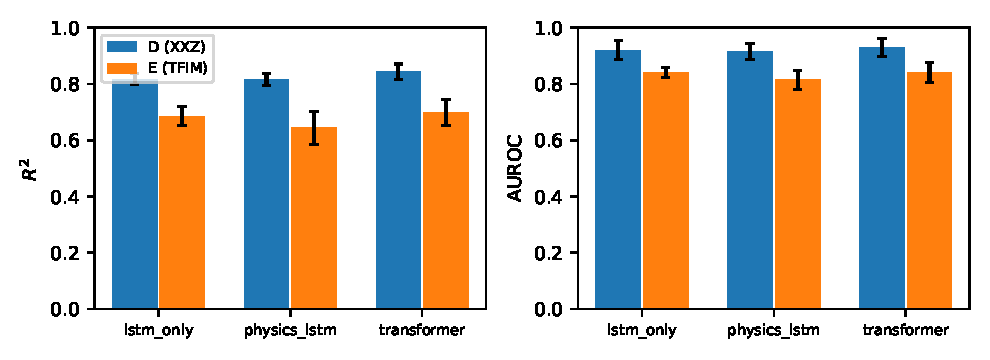
\includegraphics[width=\columnwidth]{fig_r1_ablation}
  \caption{Ablation of Table~\ref{tab:e1_2}; bars are means, whiskers one
    standard deviation over three seeds.}
  \label{fig:e6a}
\end{figure}

The Transformer is the best model on both scenarios
(Table~\ref{tab:e1_2}, Fig.~\ref{fig:e6a}) and beats both BiLSTM variants
in every seed: by $0.026 \pm 0.021$ and $0.028 \pm 0.007$ on XXZ, and by
$0.013 \pm 0.011$ and $0.055 \pm 0.018$ on TFIM (against the BiLSTM
without and with the prior). Every learned variant beats
\texttt{physics\_only} by a wide margin.
The physics prior does not help the BiLSTM: on XXZ the residual model and
the same network without the prior are level ($-0.002 \pm 0.020$), on
TFIM the residual model is worse in every seed ($-0.042 \pm 0.027$).

The large negative $R^2$ of \texttt{physics\_only} reflects the form of
the estimator rather than the physics: $-1/\hat s$ diverges as
$\hat s \to 0^-$ and the implementation returns $t_\mathrm{max}$ for
$\hat s \geq 0$, so a few windows on oscillating coherence dominate a
squared-error metric. Its MAE ($1.75 \pm 0.83$ on D, $2.77 \pm 0.74$ on
E) is $3.5$--$3.8$ times that of the Transformer.

\subsection{Measurement noise}
\label{sec:e3}

A \texttt{physics\_lstm} trained on clean D+E data is evaluated with
Gaussian noise of standard deviation $\sigma$ added to every observable
(Table~\ref{tab:e3_2}).

\begin{table}[h]
\centering
\caption{Noise robustness on D+E (mean $\pm$ s.d.\ over three
  seeds).\label{tab:e3_2}}
\small
\begin{tabular}{rccc}
\toprule
$\sigma$ & $R^2$ & MAE & AUROC \\
\midrule
0.00 & $0.493 \pm 0.121$ & $0.587 \pm 0.064$ & $0.775 \pm 0.033$ \\
0.01 & $0.529 \pm 0.101$ & $0.583 \pm 0.079$ & $0.774 \pm 0.046$ \\
0.02 & $0.489 \pm 0.064$ & $0.589 \pm 0.087$ & $0.770 \pm 0.036$ \\
0.05 & $0.498 \pm 0.058$ & $0.585 \pm 0.104$ & $0.758 \pm 0.064$ \\
0.10 & $0.420 \pm 0.164$ & $0.630 \pm 0.083$ & $0.697 \pm 0.064$ \\
\bottomrule
\end{tabular}
\end{table}

Up to $\sigma = 0.05$ neither metric changes beyond the seed-to-seed
spread. Paired within each seed, going from $\sigma = 0$ to
$\sigma = 0.10$ changes $R^2$ by $-0.074 \pm 0.126$ (per seed $-0.175$,
$-0.112$, $+0.065$), so the effect on $R^2$ is not resolved, and lowers
AUROC in every seed ($-0.078 \pm 0.037$).

\subsection{One model for both systems}
\label{sec:e11a}

A Transformer is trained on the D+E mixture and scored on each system
(Table~\ref{tab:r3}).
Only the window length differs between the two arms.

\begin{table}[h]
\centering
\caption{Cross-system Transformer, 500 trajectories per scenario
  (mean $\pm$ s.d.\ over three seeds).\label{tab:r3}}
\footnotesize
\setlength{\tabcolsep}{3pt}
\begin{tabular}{llccc}
\toprule
Window & Sc. & $R^2$ & MAE & AUROC \\
\midrule
20 & D & $\mathbf{0.814 \pm 0.034}$ & $0.603 \pm 0.045$ & $\mathbf{0.931 \pm 0.011}$ \\
20 & E & $\mathbf{0.703 \pm 0.034}$ & $0.760 \pm 0.038$ & $\mathbf{0.904 \pm 0.008}$ \\
50 & D & $0.755 \pm 0.015$ & $0.536 \pm 0.007$ & $0.886 \pm 0.023$ \\
50 & E & $0.505 \pm 0.025$ & $0.822 \pm 0.013$ & $0.803 \pm 0.017$ \\
\bottomrule
\end{tabular}
\end{table}

The shorter window wins on both metrics and both systems in every seed:
$\Delta R^2 = +0.058 \pm 0.028$ (XXZ) and $+0.199 \pm 0.014$ (TFIM),
$\Delta\mathrm{AUROC} = +0.045$ and $+0.100$.
At window 20 a single checkpoint serves both Hamiltonians at
$R^2 \geq 0.70$ and AUROC $\geq 0.90$.

Two checks qualify this result.
First, the model is scored on fresh trajectories of the configurations
it was trained on; scoring it instead on disjoint configurations from a
different generator seed changes $R^2$ by $-0.000 \pm 0.009$ on XXZ and
$+0.015 \pm 0.059$ on TFIM, so configuration overlap does not inflate
the numbers.
Second, for the residual model trained on the same mixture, doubling
the training set to 1{,}000 trajectories per scenario raises $R^2$ by
$+0.023 \pm 0.025$ on XXZ (in every seed) and by $+0.010 \pm 0.028$ on
TFIM (sign varying); at 1{,}000 trajectories it reaches
$0.815 \pm 0.015$ and $0.673 \pm 0.018$.

\subsection{TFIM coupling sweep}
\label{sec:e7c}

With $h = 1$, the infinite TFIM chain has its quantum phase transition
at $J = h$ \cite{Pfeuty1970,Sachdev2011}.
We train a Transformer separately at each
$J \in \{0.2, 0.5, 0.8, 1.0, 1.2, 1.5, 2.0\}$ (200 trajectories each;
Table~\ref{tab:r5}).

\begin{table}[h]
\centering
\caption{Transformer trained and scored at fixed $J$ (mean $\pm$ s.d.\
  over eight seeds).\label{tab:r5}}
\footnotesize
\setlength{\tabcolsep}{4pt}
\begin{tabular}{rccc}
\toprule
$J$ & $R^2$ & MAE & AUROC \\
\midrule
0.2 & $0.793 \pm 0.094$ & $0.54 \pm 0.12$ & $0.93 \pm 0.04$ \\
0.5 & $0.642 \pm 0.124$ & $0.83 \pm 0.17$ & $0.87 \pm 0.06$ \\
0.8 & $0.561 \pm 0.104$ & $0.87 \pm 0.22$ & $0.84 \pm 0.03$ \\
1.0 & $0.461 \pm 0.215$ & $1.02 \pm 0.30$ & $0.83 \pm 0.06$ \\
1.2 & $0.628 \pm 0.214$ & $0.94 \pm 0.40$ & $0.83 \pm 0.11$ \\
1.5 & $0.549 \pm 0.121$ & $1.14 \pm 0.35$ & $0.77 \pm 0.05$ \\
2.0 & $0.596 \pm 0.148$ & $1.06 \pm 0.25$ & $0.80 \pm 0.07$ \\
\bottomrule
\end{tabular}
\end{table}

Predictability falls as the coupling grows and then flattens:
$J = 0.2$ beats $J = 0.8$ in every seed ($+0.232 \pm 0.082$), the
weak-coupling points average $0.718$ against $0.559$ for $J \ge 0.8$,
and MAE roughly doubles.
The transition point carries no consistent feature: $J = h$ is the
minimum in three of eight seeds, and its $z$-score against the other
points of the same sweep ranges from $-6.8$ to $+0.9$ (median $-0.8$),
the extremes coming from single outlying runs.
This is expected for $N = 2$, where the spectrum,
$E_{P=+1} = \pm\sqrt{J^2+4h^2}$ and $E_{P=-1} = \pm J$, is analytic in
$J$ and only a smooth crossover remains.

Two dynamical explanations fail direct tests.
The dissipator does not mix the parity sectors: $L$ enters
Eq.~\ref{eq:lindblad2} quadratically and $P\sigma_-P = -\sigma_-$, and
the Liouvillian commutes with the parity superoperator to machine
precision at every $J$.
Nor is the decline caused by a generic initial state superposing modes
from both sectors: preparing the state inside one sector does not reduce
it (the drop from $J \le 0.5$ to $J \ge 0.8$ changes by
$+0.011 \pm 0.085$ for $P = +1$ and $+0.116 \pm 0.191$ for $P = -1$,
paired against generic preparation).

\subsection{The target, not the dynamics}
\label{sec:r9}

The XXZ Hamiltonian is diagonal on $|00\rangle$ and $|11\rangle$ and
mixes $|01\rangle$ and $|10\rangle$ maximally for every $J$; only the
frequency depends on $J$.
The TFIM mixes $|00\rangle$ and $|11\rangle$ through the block
$\bigl(\begin{smallmatrix}2h & J\\ J & -2h\end{smallmatrix}\bigr)$, whose
eigenbasis is rotated from the computational one by
\begin{equation}
  \tan 2\theta = J/2h ,
  \label{eq:theta}
\end{equation}
an angle that grows with $J$ and saturates at $\pi/4$.
Since $T_2$ is defined through coherence \emph{in the computational
basis}, unitary evolution modulates $C(t)$ with a depth set by $\theta$,
and the first $1/e$ crossing depends on the phase of that modulation when
the decaying envelope reaches the threshold
(Fig.~\ref{fig:r9ex}).
The $\ell_1$-coherence in the eigenbasis of $H$ is insensitive to this:
there unitary evolution only rotates the phases of $\rho_{ij}$.

\begin{figure}[t]
  \centering
  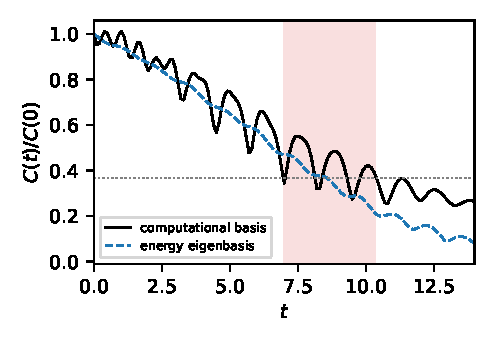
\includegraphics[width=0.9\columnwidth]{fig_r9_example}
  \caption{One TFIM trajectory at $J = 1.5$. In the energy eigenbasis
    (dashed) coherence decays smoothly; in the computational basis
    (solid) it is modulated, first crosses $1/e$ at $t = 7.0$ and is
    last above it at $t = 10.3$ (shaded).}
  \label{fig:r9ex}
\end{figure}

We measured this without training, on 150 trajectories per point drawn
as in the experiments (Table~\ref{tab:r9}): the fraction of
trajectories whose coherence returns above the threshold after first
crossing it, the mean time between the first crossing and the last
moment above threshold, and the correlation between $T_2$ and $T_2^E$,
the same crossing computed in the energy eigenbasis.

\begin{table}[h]
\centering
\caption{Target modulation (simulation only; 150 trajectories per
  point). ``Re-cross'': fraction with $C$ back above threshold after the
  first crossing; ``gap'': mean time from first crossing to last time
  above threshold; ``corr'': Pearson correlation of $T_2$ with
  $T_2^E$.\label{tab:r9}}
\footnotesize
\setlength{\tabcolsep}{3pt}
\begin{tabular}{rcccccc}
\toprule
 & \multicolumn{2}{c}{re-cross} & \multicolumn{2}{c}{gap} & \multicolumn{2}{c}{corr} \\
\cmidrule(lr){2-3}\cmidrule(lr){4-5}\cmidrule(lr){6-7}
$J$ & XXZ & TFIM & XXZ & TFIM & XXZ & TFIM \\
\midrule
0.2 & 0.00 & 0.13 & 0.00 & 0.16 & 0.977 & 0.973 \\
0.5 & 0.11 & 0.30 & 0.10 & 0.45 & 0.979 & 0.927 \\
0.8 & 0.31 & 0.56 & 0.22 & 0.82 & 0.980 & 0.890 \\
1.0 & 0.34 & 0.61 & 0.23 & 0.98 & 0.975 & 0.830 \\
1.2 & 0.48 & 0.57 & 0.37 & 1.09 & 0.954 & 0.811 \\
1.5 & 0.47 & 0.71 & 0.32 & 1.29 & 0.967 & 0.674 \\
2.0 & 0.56 & 0.75 & 0.30 & 1.28 & 0.971 & 0.676 \\
\bottomrule
\end{tabular}
\end{table}


On TFIM the re-crossing fraction and the gap grow with $J$ and saturate,
and the correlation with the envelope falls from $0.97$ to $0.67$: at
$J \ge 1.5$ the envelope explains less than half of the variance of
$T_2$, and the gap ($\approx 1.3$) is about a third of the mean $T_2$
($\approx 4.2$).
On XXZ the correlation stays above $0.95$ at every $J$ and the gaps are
four times smaller.
Across the seven $J$ values the re-crossing fraction correlates with the
trained models' $R^2$ at $r = -0.78$ ($p \approx 0.04$; Spearman
$-0.68$).
Without dissipation the modulation alone almost never takes $C$ below
threshold ($\le 0.3\%$ of random states), so the target is set by
dissipation but its \emph{timing} is shifted by the unitary part.

This evidence is correlational: seven points, and the modulation grows
with $J$ together with the overall energy scale $\sqrt{J^2+4h^2}$.
The direct test is to repeat the coupling sweep with $T_2^E$ as the
target and everything else unchanged---same configurations, seeds, model
and training, inputs still in the computational basis
(Table~\ref{tab:r10}, Fig.~\ref{fig:r9J}).

\begin{table}[h]
\centering
\caption{Coupling sweep with the computational-basis target ($T_2$,
  Table~\ref{tab:r5}) and the energy-basis target ($T_2^E$); mean
  $\pm$ s.d.\ over the same eight seeds.\label{tab:r10}}
\footnotesize
\setlength{\tabcolsep}{2.5pt}
\begin{tabular}{rcccc}
\toprule
 & \multicolumn{2}{c}{$R^2$} & \multicolumn{2}{c}{MAE} \\
\cmidrule(lr){2-3}\cmidrule(lr){4-5}
$J$ & $T_2$ & $T_2^E$ & $T_2$ & $T_2^E$ \\
\midrule
0.2 & $0.793 \pm 0.094$ & $0.861 \pm 0.038$ & $0.54 \pm 0.12$ & $0.48 \pm 0.10$ \\
0.5 & $0.642 \pm 0.124$ & $0.811 \pm 0.134$ & $0.83 \pm 0.17$ & $0.47 \pm 0.12$ \\
0.8 & $0.561 \pm 0.104$ & $0.787 \pm 0.140$ & $0.87 \pm 0.22$ & $0.49 \pm 0.14$ \\
1.0 & $0.461 \pm 0.215$ & $0.799 \pm 0.085$ & $1.02 \pm 0.30$ & $0.45 \pm 0.06$ \\
1.2 & $0.628 \pm 0.214$ & $0.804 \pm 0.100$ & $0.94 \pm 0.40$ & $0.47 \pm 0.14$ \\
1.5 & $0.549 \pm 0.121$ & $0.852 \pm 0.099$ & $1.14 \pm 0.35$ & $0.41 \pm 0.14$ \\
2.0 & $0.596 \pm 0.148$ & $0.835 \pm 0.048$ & $1.06 \pm 0.25$ & $0.47 \pm 0.13$ \\
\bottomrule
\end{tabular}
\end{table}

\begin{figure}[t]
  \centering
  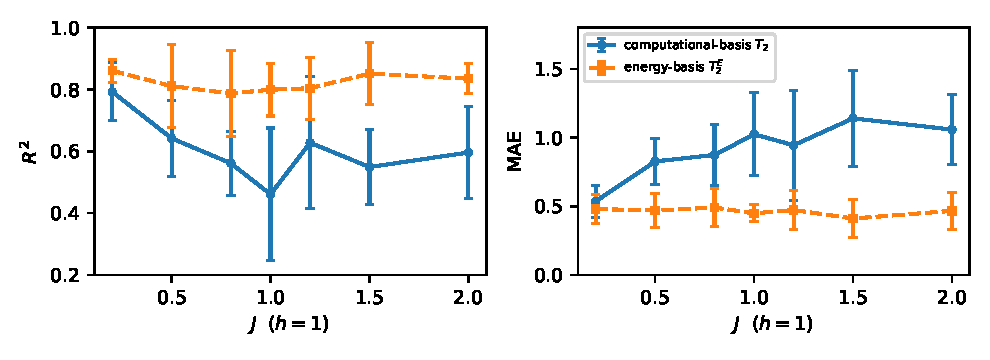
\includegraphics[width=\columnwidth]{fig_r5_r9_J}
  \caption{Coupling sweep with the two targets of Table~\ref{tab:r10};
    whiskers are one standard deviation over eight seeds.}
  \label{fig:r9J}
\end{figure}

With the energy-basis target the predictability no longer depends on
the coupling. The drop in $R^2$ from weak ($J \le 0.5$) to strong
coupling ($J \ge 0.8$) is $0.158 \pm 0.066$ with the computational-basis
target, positive in all eight seeds, and $0.020 \pm 0.072$ with the
energy-basis target, with the sign varying; it shrinks in seven of eight
seeds. The rise in MAE over the same range is $0.33 \pm 0.21$ (positive
in every seed) against $-0.02 \pm 0.13$. $R^2$ is higher with the
energy-basis target in 49 of 56 seed--$J$ pairs.
The loss of predictability with coupling is thus mostly a property of
the target: what the model cannot predict at strong coupling is the
phase of the unitary modulation at the threshold crossing, not the
dissipative decay.

% --------------------------------------------------------------------------
\section{Discussion}
\label{sec:discussion}

\paragraph{The physics prior on two qubits.}
In the single-qubit case the slope-based estimate gives the BiLSTM a
clear advantage over the same network without it, and the residual model
is the most accurate model there \cite{Paper1Brusnikin}.
On two qubits the formula is not merely imprecise but structurally
wrong: oscillating coherence breaks the assumption that $\log C$ is
linear over the window.
Unlike a PINN \cite{Raissi2019}, where a physics term is a soft penalty,
our prior is part of the output; when it is wrong, the network has to
undo it through $\delta T$.
The gate removes it on the worst windows, and the residual model ends up
level with the same network without the prior on XXZ and worse on TFIM
(Table~\ref{tab:e1_2}).
The recommended model for two qubits is the Transformer: it is the most
accurate and the most stable across seeds.

\paragraph{What limits TFIM.}
Most of the TFIM ceiling is not a property of the model or of the data
size but of the target (Sec.~\ref{sec:r9}): the first crossing of a
basis-dependent quantity is partly a matter of oscillation phase, and
with an energy-basis target the error stops growing with the coupling.
The practical lesson is to define the decoherence time through a
quantity that the Hamiltonian does not modulate---the coherence in the
energy eigenbasis, or a basis-independent measure---whenever the
Hamiltonian is not diagonal in the measurement basis.
Whether the remaining modulation could be predicted from the window is
open; the oscillation phase is fixed by the initial state, but the model
does not see two-body correlators.

\paragraph{Limitations.}
All data are simulated, with $\gamma(t)$ drawn from a smooth polynomial
family; real devices add non-Markovian noise and correlated readout
errors.
With $N = 2$ no statement about phase transitions is possible.
Test sets are small (about 40 trajectories per scenario, 18 per $J$),
which limits the resolution of every comparison to the replicated
spreads quoted.

\paragraph{Open questions.}
\begin{enumerate}
  \item The energy-basis target for XXZ and for the cross-system model.
  \item Two-body correlators and entanglement measures (concurrence
    \cite{Wootters1998}, negativity) as inputs, or entanglement as an
    alternative target.
  \item Extension to three and four qubits.
\end{enumerate}

% --------------------------------------------------------------------------
\section{Conclusion}

\begin{enumerate}
  \item The single-qubit conclusion does not transfer: on two qubits the
    Transformer is best ($R^2 = 0.843 \pm 0.028$ on XXZ,
    $0.699 \pm 0.045$ on TFIM) and beats both BiLSTM variants in every
    seed; the residual model is no better than the same BiLSTM without
    the prior, and on TFIM it is worse.
  \item A single Transformer with a 20-step window serves both systems
    at $R^2 = 0.814$ and $0.703$, AUROC $0.931$ and $0.904$; the shorter
    window beats a longer one on both metrics in every seed.
  \item Measurement noise up to $\sigma = 0.05$ changes neither metric
    beyond the seed-to-seed spread; at $\sigma = 0.10$ AUROC falls in
    every seed.
  \item On TFIM predictability falls with coupling and saturates; the
    transition point is not special.
  \item The decline is consistent with modulation of the target: the
    computational-basis coherence that defines $T_2$ is modulated by the
    Hamiltonian with a depth set by $\tan2\theta = J/2h$, and the
    resulting ambiguity of the crossing time tracks the loss in $R^2$.
    With the decoherence time defined in the energy eigenbasis the
    dependence on coupling disappears (drop in $R^2$ $0.020 \pm 0.072$
    against $0.158 \pm 0.066$, eight seeds).
\end{enumerate}

% --------------------------------------------------------------------------
\section*{Data availability}
All data in this paper are simulated; no experimental data were used.
Every table is produced by the accompanying code from the trajectory
generator described in Sec.~\ref{sec:method}, and the result files behind
each table are retained alongside it.

\section*{Code availability}
The simulation, training, evaluation and figure-generating code, together
with the result files behind every table, is publicly available at
\url{https://github.com/Mobo140/decoherence}.
In the repository the ablation and noise runs are experiment E6, the
coupling sweep E7 and the cross-system runs E11; their three-seed
replications are R1, R8, R5 and R3, the configuration-overlap check R4,
the parity-sector test R6, the target-modulation probe R9 and the
coupling sweep with the energy-basis target R10.

\section*{Reproducibility}
All runs are seeded end to end: the sampled system configurations, each
trajectory's initial state, the window sampling and split, and the
network initialisation and batch order.
A run started from an empty trajectory cache is deterministic.
Results were produced with Python~3.12.1, NumPy~2.4.4, SciPy~1.17.1,
QuTiP~5.2.3 and PyTorch~2.11.0 on CPU, with seeds $\{42,43,44\}$.

\section*{Competing interests}
\needspaste{competing-interests declaration --- usually ``The author
declares no competing interests.''}

\section*{Funding}
\needspaste{funding statement, or ``This research received no specific
grant from any funding agency.''}

% --------------------------------------------------------------------------
\bibliographystyle{unsrt}
\begin{thebibliography}{13}

\bibitem{Paper1Brusnikin}
N.~Brusnikin,
``Physics-Informed Early Warning of Quantum Decoherence in Single-Qubit
  Systems Under Unknown Time-Dependent Dissipation,''
manuscript in preparation (2026). [companion paper]

\bibitem{qutip}
J.~R.~Johansson, P.~D.~Nation, and F.~Nori,
``QuTiP: An open-source Python framework for the dynamics of open
  quantum systems,''
\textit{Comput.\ Phys.\ Commun.}\ \textbf{183}, 1760--1772 (2012).

\bibitem{TransformerLindblad2025}
C.-S.~Chen and E.-J.~Kuo,
``Unraveling quantum environments: Transformer-assisted learning in
  Lindblad dynamics,''
\textit{Phys.\ Rev.\ A}\ \textbf{112}, 042227 (2025); arXiv:2505.06928.

\bibitem{Raissi2019}
M.~Raissi, P.~Perdikaris, and G.~E.~Karniadakis,
``Physics-informed neural networks: A deep learning framework for
  solving forward and inverse problems involving nonlinear partial
  differential equations,''
\textit{J.\ Comput.\ Phys.}\ \textbf{378}, 686--707 (2019).

\bibitem{Lidar2013}
D.~A.~Lidar and T.~A.~Brun (eds.),
\textit{Quantum Error Correction},
Cambridge University Press, 2013.

\bibitem{Pfeuty1970}
P.~Pfeuty,
``The one-dimensional Ising model with a transverse field,''
\textit{Ann.\ Phys.}\ \textbf{57}, 79--90 (1970).

\bibitem{Sachdev2011}
S.~Sachdev,
\textit{Quantum Phase Transitions},
2nd ed., Cambridge University Press, 2011.

\bibitem{Lindblad1976}
G.~Lindblad,
``On the generators of quantum dynamical semigroups,''
\textit{Commun.\ Math.\ Phys.}\ \textbf{48}, 119--130 (1976).

\bibitem{Breuer2002}
H.-P.~Breuer and F.~Petruccione,
\textit{The Theory of Open Quantum Systems},
Oxford University Press, 2002.

\bibitem{YuEberly2009}
T.~Yu and J.~H.~Eberly,
``Sudden death of entanglement,''
\textit{Science}\ \textbf{323}(5914), 598--601 (2009).

\bibitem{Wootters1998}
W.~K.~Wootters,
``Entanglement of formation of an arbitrary state of two qubits,''
\textit{Phys.\ Rev.\ Lett.}\ \textbf{80}, 2245--2248 (1998).

\bibitem{Vaswani2017}
A.~Vaswani, N.~Shazeer, N.~Parmar, J.~Uszkoreit, L.~Jones,
A.~N.~Gomez, {\L}.~Kaiser, and I.~Polosukhin,
``Attention is all you need,''
\textit{Advances in Neural Information Processing Systems (NeurIPS)}
  \textbf{30} (2017); arXiv:1706.03762.

\bibitem{HochreiterSchmidhuber1997}
S.~Hochreiter and J.~Schmidhuber,
``Long short-term memory,''
\textit{Neural Computation}\ \textbf{9}(8), 1735--1780 (1997).

\bibitem{Fawcett2006}
T.~Fawcett,
``An introduction to ROC analysis,''
\textit{Pattern Recognition Letters}\ \textbf{27}(8), 861--874 (2006).

\end{thebibliography}

\end{document}
